\documentclass[11pt]{amsart}

\usepackage{geometry}  
\geometry{letterpaper} 
\usepackage{graphicx}
%\usepackage[backend=bibtex]{biblatex}
\usepackage{array}
\usepackage{amssymb}
\usepackage{amsmath}
\usepackage{amsthm}
\usepackage{graphicx}
\usepackage[parfill]{parskip} 
\usepackage[utf8]{inputenc}
\usepackage[english]{babel}
\usepackage{tikz}
\usetikzlibrary{arrows}
\usepackage{tikz-cd}
\usepackage[noend]{algpseudocode}
\usepackage{caption}
\usepackage{subcaption}
\usepackage{fancyhdr}
\usepackage{enumitem}
\usepackage[super]{nth}
\usepackage{pstricks}
\usepackage{comment}
\usepackage{bbm}

\usepackage[colorlinks=true,linkcolor=blue]{hyperref}


\pagestyle{fancy}
\lhead{}
\chead{}
\rhead{}
\lfoot{}
\cfoot{\thepage}
\rfoot{}
\renewcommand{\headrulewidth}{0pt}
\setlength{\footskip}{50pt}

\makeatletter
\def\BState{\State\hskip-\ALG@thistlm}
\makeatother

\theoremstyle{plain}
\newtheorem{thm}{Theorem}[section]

\newtheorem{cor}[thm]{Corollary}

\newtheorem{prop}[thm]{Proposition}

\newtheorem{dfn}[thm]{Definition}

\newtheorem{lem}[thm]{Lemma}

\newtheorem{ex}[thm]{Example}

\newtheorem{conj}[thm]{Conjecture}

\newtheorem{algorithm}[thm]{Algorithm}

\newtheorem*{rem}{Remark}
\newtheorem{assumption}[thm]{Assumption}

\newcommand{\Rom}[1]
    {\MakeUppercase{\romannumeral #1}}

\graphicspath{ {images/} }

\pgfdeclarelayer{edgelayer}
\pgfdeclarelayer{nodelayer}
\pgfsetlayers{edgelayer,nodelayer,main}


\tikzstyle{Dashed Line}=[-, draw=blue, dashed]
\tikzstyle{none} = []
\tikzstyle{new edge style 1}=[<->, thick]
\tikzstyle{new edge style 2}=[{<- left hook}]



\newcommand{\C}[1]{(\mathbb{C}^\times)^#1}
\newcommand{\mb}[1]{\mathbb{#1}}

\begin{document} 


\section{Introduction}

All varieties we consider are normal and projective. Here we give an algorithm to classify Log Del Pezzos admitting a $\mathbb{C}^\times$ action with only log terminal singularities. A variety $X$ of dimension $n$ which admits a torus action of dimension $n-k$ is referred to as complexity $k$. Here complexity 0 is the study of purely toric varieties, and complexity $n$ is the study of varities with no possible torus action. This provides essentailly a way of grading the difficulty of your problem. Significant progress has been made on this problem before: S\"{u}ss \cite{Suss} classifies log del Pezzo surfaces admitting said action with Picard rank one and index less than 3. Huggenberger \cite{Huggenberger} classifies the anticanonical complex of the Cox ring of log del Pezzo surfaces with index 1, this classification was later finished by Ilten, Mishna and Trainor \cite{IMT} with a view towards higher dimension. This was achieved by looking at polarised complexity one log del Pezzo surfaces. We will show their work fits into our algorithm. 
\\
\\
\section{Polyhedral divisors}
Recall that a toric variety is a  normal variety of dimension $n$ containing a dense torus $\C{n}$ with the natural action extending to the variety, there is a one to one correspondence between these varieties and fans inside a lattice $N \cong \mathbb{Z}^n$ upto GL$_2(\mathbb{Z})$, \cite{Cox}.
Altman et.al \cite{Altmann} establish a similar correspondence for varieties with $T = \C{{ n-k}}$ actions where $k \leq n$. We say that this is a torus action of complexity $k$. They introduce the notion of a polyhedral divisor to recover some of the geometry that a fan encodes in the toric case. In general this applies for any complexity, however the behaviour is easiest to describe in the toric case, then complexity one until you reach the full general case.


Given $X$, a variety with dimension $n$ admitting of the torus $ T = (\mathbb{C}^*)^{n-1}$ action, we can take a Chow quotient $Y$ of $X$ by $T$, essentially a GIT quotient followed by normalisation.  We see that $Y$ will be a variety of dimension $k$, we can resolve this map to $\tilde{X}$ getting the following diagram

\[
\begin{tikzcd}
X \arrow[rd, dotted] & \tilde{X} \arrow[l] \arrow[d]\\
& Y
\end{tikzcd}
\]

Here $Y \cong C$ is a normal curve. In this thesis we will primarily be interested in the case where $C \cong \mathbb{P}^1$. We start by introducing the notion of a tail cone of a given polyhedral cone. This is given $F$ a polyhedral subdivision such that the tail cone $\delta$ is the set of $v \in N$ such that $F_i$ is invariant under the translation, i.e $\delta = \{ v |\, v(F) subset F \}$.
\begin{dfn}
Let $C$ be a nonsingular curve then we define a polyhedral divisor to be the pair $(\mathcal{D} = \sum_{i = 1}^k F_i \otimes P_i$, $\delta)$ where
\begin{itemize}
\item $P_i \in C$ are divisors on $C$ 
\item $F_i$ is a polyhedron contained in $N_\mathbb{Q} \cong \mathbb{Q}^{n-1}$ and all $F_i$ have tail cone $\delta \subset N$.  We allow the cone $F_i$ to be $\varnothing$.
\end{itemize}
Given an element $v \in M$, the dual lattice of $N$, and the polyhedral divisor $\mathcal{D}$ we define
\[
\mathcal{D}(v) = \sum \min_{u \in F_i} \langle u, v \rangle P_i
\]
This is defined as a divisor on the following curve
\[
Y_\mathcal{D} = C - \{P_j\}_{j \text{ where } F_j = \varnothing}
\]
\end{dfn}

This defines a divisor on a subset of $C$. We insist that $\mathcal{D}$ satisfies the following conditions:
\begin{enumerate} 
\item $\mathcal{D}(u)$ is Cartier for all $u \in \delta^\vee $
\item $\mathcal{D}(u)$ is semiample for all $u \in \delta^\vee$
\item $\mathcal{D}(u)$ is big for all $u$ in the relative interior of $\delta^\vee$
\end{enumerate}
This is to ensure that it gives an $n$-dimensional variety, and to ensure that it is separated \cite{PS}.


We can now calculate the associated affine varieties $X$ and $\tilde{X}$ by taking respectively Spec/ RelSpec${_C}$ of the graded ring
\[
\bigoplus_{v \in \delta^\vee} \mathcal{O}_{Y_\mathcal{D}} ( \mathcal{D}(v))
\]
This gives us an affine variety with $T = \text{Spec } \mathbb{C}[M]$ acting by torus action. Analogous to the toric case, if $F_i \subset F_j$ is a face then we have
\[
\bigoplus_{v \in \delta^\vee} \mathcal{O}_{Y_\mathcal{D}}( \mathcal{D}_{F_j}(v)) \subset \bigoplus_{v \in \delta^\vee} \mathcal{O}_{Y_\mathcal{D}}( \mathcal{D}_{F_i}(v)) 
\]
This corresponds to an inclusion of schemes. We make the following comment that taking a divisor 
\[ 
\mathcal{D} = \sum_{i = 1}^n F_i \otimes P_i + \varnothing \otimes P_{n+1}
\]
is the same as taking the divisors 
\[
\mathcal{D}_i = F_i \otimes P_i  + \sum_{j=1, \, j \neq i} \varnothing \otimes P_j
\]
and then glueing these affine varieties together along the affine patch defined by $C-P_i - P_j$ for all $P_i$, $P_j$. We say that if the tail cone of a polyhedral divisor $\mathcal{D}$ is non zero and there is no point $P$ such that $\mathcal{D}|_P = \varnothing$ then $\mathcal{D}$ is marked. The variety $\widetilde{X}$ is defined to be the variety such that the cone is not marked.


We now introduce the notion of a polyhedral fan. Consider a collection of polyhedral divisors $\mathcal{S} = \{ \mathcal{D}_i \}$ such that the tail cones form a fan in the sense of toric geometry, we call this the tail fan. Given $\mathcal{S} \ni \mathcal{D}_i = \sum \sigma^i_j \otimes P_j$ then  we can make the divisor $\mathcal{D} = \sum \tau_j \otimes P_j$ where $\tau_j$ a face of each cone corresponding to a face of the tail cone. If $\mathcal{D} \in \mathcal{S}$ for all possible faces of all the tail cone, then this is a polyhedral fan. As this is stated above this makes no mention of how this behaves with respect to a divisor $\mathcal{D} = \sum \sigma_i \otimes P_i + \varnothing \otimes P$. 
To do this we add that if given a face of the tail fan $\delta$ there is associated polyhedral divisor $\mathcal{D} = \sum \sigma_i \otimes P_i$ with $\delta$ as its tail cone. We then insist that if a cone in the tail fan is not marked then every face of the cone is also not marked. If the collection $\mathcal{S}$ satisfies these conditions then we call it a polyhedral fan.


Given a complexity one projective variety $X$ over a curve $C$ this corresponds to a polyhedral fan with the tail fan spanning $N$. Analaously to the case in cones, the variety $\widetilde{X}$ is defined to be the complexity one variety with the same tail fan and polyhedral divisors however every cone is not marked. The action of the $(\mb{C}^\times)^{n-1}$ on $\widetilde{X}$ corresponds to a fibration over $C$ with general fiber $X_t$ equal to the toric variety defined by the tail fan. The degenerate fibers are then described by the polyhedral fans. 



In the case of surfaces of complexity one we often use the notation of fansy divisors as set out in \cite{Suss}. This follows the key notion that in the case of $n=2$ and $k=1$ we have that every tail fan is either $0$, $\mathbb{Z}_{\geq 0 }$ or $\mathbb{Z}_{\leq 0}$ We have $n$ subdivisions of $N \cong \mathbb{Z}$, these should be viewed as the polyhedral divisors over these $n$ points. Note that if we have a closed interval in any of subdivisions this will have tail fan zero and these give rise to a cyclic quotient singularity, with a nice torus quotient, i.e the map to $\tilde{X}$ is a contraction to a point. It is the intervals $[a_1, \infty )$ which provide difficulty, if as polyhedral divisors these are all of the form 
\[
\mathcal{D}_i = [a_i, \infty) \otimes P_i + \sum_{\substack{j = 1 \\ j \neq i}}^n \varnothing \otimes P_j
\]
\textbf{Change this paragraph}
Then this gives rise to a nice quotient map down base curve with respect to the torus action, i.e  the map to $\tilde{X}$ is a local isomorphism. If this is not the case however, then we are left with a bad quotient. In the surface case, there are the only two cases that can occur. In the language of fansy divisors we say if we mean the latter case we denote it with $\mathbb{Q}^+$, if we mean the other the earlier case, we do no denote it at all. In this way fansy divisor uniquely specify polyhedral fans.
\\
\\
\section{ Example}

\begin{ex}\rm
The first is the polyhedral divisor given by the unmarked polyhedral divisor $[0, 1] \otimes P_0$ over $Y = \mb{P}^1$. 
The tail cone $\delta$ is equal to $0$. We will show how we can construct from this an affine variety $X$. We denote the polyhedral divisor by $\mathcal{D}$. So the dual of the tail cone $\hat{\delta}$ is the lattice $M$ itself. Given an element $ m >0$ of $M$ we have $\mathcal{D}(m) = -mP_0$ as the minimum value is obtained on $-1$. If $m <0$ we get $\mathcal{D}(m) = mP_0$  as the minimum is attained on 1. Finally if $n=0$ we get $\mathcal{D}(m) = 0$ as a divisor on $\mathbb{A}^1$ as the function is 0 everywhere. 


Hence we have the $M$ graded ring
\[
\bigoplus_{m \in M} \mathcal{O}_{\mathbb{A}^1}(-|m|P)
\]
In degree 0 the ring is generated by the constant function on $\mb{A}^1$ which we denote $x$ and the function $y$ which is zero at the origin. We note that the function $1$ in degree 0 is the multiplicative identity of our ring. In degree one every element is of the form $f ( a_0 x + a_1 y + a_2 y^2 + \dots  a_n y^n)$, here $f$ is the same function on $\mb{A}^1$ as $y$ but now in degree 1. Every element of degree $m>0$ is of the form $f^m ( a_0 x + a_1 y + a_2 y^2 + \dots  a_n y^n)$. Hence this ring is generated in degree 1. The calculation on the ring graded in negative degree is exactly the same, except with a function $g$.  We note that $fg = y^2$ as $f$ and $g$ are both equal to $y$ as functions on $\mb{A}^1$. We finally discuss the function $x$. Given a function $F \in \mb{C}(X)$, then $F = \sum F_i \chi^{m_i}$, here the $F_i$ are functions on the curve $Y$ and $\chi^{m_i}$ are monomials in the lattice $M$. By construction the function $x = \mathbbm{1}_{Y} \, \chi^0$, hence $x$ is the constant function on the variety. Hence we get the ring $\mathbb{C}[f,  \, g, \, y]/ (fg=y^2)$, so an $A_1$ singularity.
\end{ex}

We can more generally describe what occurs with divisors of the $[\frac{a}{b}, \, \frac{c}{d}] \otimes P_0$. We note that the tail cone $\delta$ is always 0 and so the dual tail cone is all of $M$. From the definitions we get the ring $R = \oplus_M R_m$ where
\[
R_n = 
\left\{
\begin{array}{cc}
\mathcal{O}_{\mb{A}^1} ( \frac{ma}{b}P) & \text{if } m \geq 0  \vspace{0.2cm} \\
\mathcal{O}_{\mb{A}^1} ( \frac{mc}{d}P) & \text{if } m \leq 0 
\end{array}
\right.
\]

We can associate the monomial $z^u \chi^v$ with the lattice point $(u,v)$ inside a two dimensional monomial lattice. This gives rise to a cone $\sigma$. The set of monomials with poles of order at worst $\frac{a}{b}$ gives rise to the vector $(a, -b)$. Similarly the other side of the graded ring gives rise to the vector $(-c, d)$. These are boundaries $\sigma$, this means that as toric variety they can be described as the cone $(a,b)$, $(c,d)$ inside the lattice $N$ with torus action corresponding to $(1,0)$.  Hence we get a toric variety of the form $\frac{1}{ad-bc}(u,v)$.


\begin{ex}\rm
We now show how this behaves in the case of a divisor with tail cone $\delta = [0, \, \infty)$. Consider the divisor $\mathcal{D} = \left[\frac{1}{2}, \, \infty \right) \otimes P_0 + \left[\frac{1}{2}, \, \infty \right) \otimes P_1 + \left[\frac{-1}{2}, \, \infty \right) \otimes P_2$ over $\mb{P}^1$ with coordinates $x_1, \, x_2$. Here the varieties $X$ and $\widetilde{X}$ are different. To start with, we look at how to construct $X$. For simplicity we assume $P_0 = (1; \, 0)$, $P_1 = (1; \, 1)$ and $P_2 = (0; \, 1)$.

The tail cone is $\delta = [0, \, \infty)$ so $\hat\delta = [0, \, \infty)$. By calculating $\mathcal{D}(m)$ we get the following ring
\[
\bigoplus_{m \in M|_{\geq 0}} \mathcal{O}_{\mb{P}^1} \left( \frac{m}{2} P_0 + \frac{m}{2} P_1 + \frac{-m}{2} P_2 \right)
\]
Once again in degree 0 we get the constant function. In degree one we get no functions. In degree 2 we get 2 functions $\frac{x_2}{x_1} \chi^2 $ and $\frac{x_2}{x_1-x_2} \chi^2$ denote these $u$ and $v$. In degree 3 we get the function $\frac{x_2^2}{x_1(x_1-x_2)} \chi^3 $ denote this by $w$. We then have the relations $w^2 = uv(v-u)$. This gives rise to a $D_4$ singularity.  

To calculate $\widetilde{X}$ we do all these calculations as relative spec. In particular this means we can our above graded ring with the following three graded rings
\[
\bigoplus_{m \in M|_{\geq 0}} \mathcal{O}_{(\mb{P}^1 - P_i - P_j)} \left( \frac{m}{2} P_0 + \frac{m}{2} P_1 + \frac{-m}{2} P_2 \right)
\]
For all choices of $i$ and $j$. We then glue together on the intersection. Calculating in the case $i=1$ and $j =2$. We have
\[
\bigoplus_{m \in M|_{\geq 0}} \mathcal{O}_{(\mb{P}^1 - P_1 - P_2)} \left( \frac{m}{2} P_0 + \frac{m}{2} P_1 + \frac{-m}{2} P_2 \right) \cong \bigoplus_{m \in M|_{\geq 0}} \mathcal{O}_{(\mb{A}^1 - P_1)} (\frac{m}{2}P_0)
\]
This gives us the ring $\mb{C}[x, \frac{1}{x+1}, \frac{1}{x}\chi^2, \chi^1] = \mb{C}[u,v,w,t]/[v(u+1) = 1, \, uw = t^2]$. Hence this is an $A_1$ singularity. The calculations on the other 3 patches are the same, so we have taken the partial resolution of the $D_4$ singularity by extracting the trivalent curve. 
\end{ex}


\begin{ex}\rm
Consider the following polyhedral fan with marking $\mb{Q}^\pm$
\[
\begin{tikzpicture}
	\begin{pgfonlayer}{nodelayer}
		\node [style=none] (0) at (-7, 4) {};
		\node [style=none] (1) at (-7, 4.25) {};
		\node [style=none] (2) at (-7, 3.75) {};
		\node [style=none] (3) at (-3, 4) {};
		\node [style=none] (4) at (-3, 4.25) {};
		\node [style=none] (5) at (-3, 3.75) {};
		\node [style=none] (6) at (0, 4) {};
		\node [style=none] (7) at (-10, 4) {};
		\node [style=none] (14) at (0, 2) {};
		\node [style=none] (15) at (-10, 2) {};
		\node [style=none] (16) at (-4, 1.75) {};
		\node [style=none] (17) at (-4, 2.25) {};
		\node [style=none] (18) at (-10, 0) {};
		\node [style=none] (19) at (-6, 0.25) {};
		\node [style=none] (20) at (-6, -0.25) {};
		\node [style=none] (21) at (0, 0) {};
		\node [style=none] (22) at (-7, 3.25) {};
		\node [style=none] (23) at (-7, 3.25) {-1};
		\node [style=none] (24) at (-3, 3.25) {1};
		\node [style=none] (25) at (-4, 1.25) {};
		\node [style=none] (26) at (-4, 1.25) {$\frac{1}{2}$};
		\node [style=none] (27) at (-6, -0.75) {};
		\node [style=none] (28) at (-6, -0.75) {$-\frac{1}{2}$};
		\node [style=none] (29) at (-10, -2) {};
		\node [style=none] (30) at (0, -2) {};
		\node [style=none] (31) at (-5, -2) {};
		\node [style=none] (32) at (-5, -2.75) {};
		\node [style=none] (33) at (-5, -2.75) {0};
		\node [style=none] (34) at (2, 5) {};
		\node [style=none] (35) at (2, -3) {};
		\node [style=none] (36) at (1.5, 1) {$\mathbb{P}^1$};
		\node [style=none] (37) at (2.5, -2) {};
		\node [style=none] (38) at (2.5, -2) {$P_{\text{gen}}$};
		\node [style=none] (39) at (2.5, 0) {$P_\infty$};
		\node [style=none] (40) at (2.5, 2) {};
		\node [style=none] (41) at (2.5, 2) {$P_1$};
		\node [style=none] (42) at (2.5, 4) {$P_0$};
		\node [style=none] (43) at (-5, -2.25) {};
		\node [style=none] (44) at (-5, -1.75) {};
	\end{pgfonlayer}
	\begin{pgfonlayer}{edgelayer}
		\draw (1.center) to (2.center);
		\draw (4.center) to (5.center);
		\draw (17.center) to (16.center);
		\draw (19.center) to (20.center);
		\draw [style=new edge style 1] (21.center) to (18.center);
		\draw [style=new edge style 1] (15.center) to (14.center);
		\draw [style=new edge style 1] (7.center) to (6.center);
		\draw [style=new edge style 1] (29.center) to (30.center);
		\draw [style=new edge style 1] (34.center) to (35.center);
		\draw (43.center) to (44.center);
	\end{pgfonlayer}
\end{tikzpicture}
\]
We now go through each polyhedral divisor and calculate the associated rings. 
There are three polyhedral divisors contained inside this polyhedral fan which are one dimensional cones. There are three polyhedral divisors which correspond to two dimensional cones. 

\begin{enumerate}[label =\alph*)]
\item The unmarked polyhedron $[-1, \, 1]$
\item The marked cone $1\otimes P_0 + \frac{1}{2} \otimes P_1 + \frac{-1}{2} \otimes P_\infty$ with tail cone $[0,\, \infty)$.
\item The marked cone $1\otimes P_0 + \frac{1}{2} \otimes P_1 + \frac{-1}{2} \otimes P_\infty$ with tail cone $(-\infty, \, 0]$.
\end{enumerate}

In case $a$ the tail cone $\delta$ is equal to $0$. We denote the polyhedral divisor by $\mathcal{D}$. So the dual of the tail cone $\hat{\delta}$ is the lattice $M$ itself. Given an element $ m >0$ of $M$ we have $\mathcal{D}(m) = -mP_0$. If $m <0$ we get $\mathcal{D}(m) = mP_0$ and if $n=0$ we get $\mathcal{D}(m) = 0$ as a divisor on $\mathbb{A}^1$. 

Hence we have the $M$ graded ring
\[
\bigoplus_{m \in M} \mathcal{O}_{\mathbb{A}^1}(-|m|P)
\]
In degree 0 the ring is generated by the constant function $x$ and the function $y$ which is zero at the origin. We note that the function $1$ in degree 0 is the multiplicative identity of our ring. In degree one every element is of the form $f ( a_0 x + a_1 y + a_2 y^2 + \dots  a_n y^n)$, here $f$ is the same function as $y$ but now in degree 1. Every element of degree $m>0$ is of the form $f^m ( a_0 x + a_1 y + a_2 y^2 + \dots  a_n y^n)$. Hence this is generated in degree 1. The calculation on the ring graded in negative degree is exactly the same.  Hence we get the ring $\mathbb{C}[f,  \, g, \, y]/ (fg=y^2)$, so an $A_1$ singularity.


In case $a$ the tail cone $\delta$ is equal to $[0 ,  \, \infty)$. We denote the polyhedral divisor by $\mathcal{D}$. So the dual of the tail cone $\hat{\delta}$ is $[0 ,  \, \infty) \subset M$. Given an element $ m \geq 0$ of $M$ we have $\mathcal{D}(m) = mP_0 +\frac{m}{2} P_1 + \frac{-m}{2}P_2$. 

Hence we have the $M$ graded ring
\[
\bigoplus_{m \in M|_{\geq 0}} \mathcal{O}_{\mathbb{P}^1} \left(mP_0 +\frac{m}{2} P_1 + \frac{-m}{2}P_2 \right) \cong \bigoplus_{m \in M|_{\geq 0}} \mathcal{O}_{\mathbb{P}^1} \left(\frac{m}{2} P_1 + \frac{m}{2}P_2 \right)
\]
Here the isomorphism follows via linear equivalence of divisors on $\mathbb{P}^1$.

In degree 0 we just get the constant function. In degree 1, once again it is only the constant function, denoted this by $x$. In degree 2 we have the function with a pole at $P_1$ and a zero at $P_2$, denote this by $f$ and the function $g = \frac{1}{f}$. This generates the ring hence we have $\mathbb{C}[x, \, f, \, g]/(fg = x^4)$, so an $A_3$ singularity.


Case $c$ is exactly the same as case $b$ but with the grading negative instead of positive. So it is also an $A_3$ singularity.


We finish by discussing the unmarked polyhedral divisors

\begin{enumerate}[label =\Alph*)]
\item The unmarked cone $-1 \otimes P_0$
\item The unmarked cone $1 \otimes P_0$
\item The unmarked cone $\frac{1}{2} \otimes P_1$
\item The unmarked cone $-\frac{1}{2} \otimes P_2$
\end{enumerate}

In all case the tail cone $\delta$ is equal to 0. In case $A$ have the following ring graded by $M$

\[
\bigoplus_{m \in M} \mathcal{O}_{\mathbb{A}^1}(-mP) \cong \mathbb{C}[x,\, y, \, z]/(yz = 1)
\]
Here $x$ is of degree 0, $y$ is of degree 1 and $z$ is of degree $-1$. Case $B$ is symmetrical to case $A$. 

Cases $C$ and $D$ are also symmetrical, and give rise to the rings $\mathbb{C}[x, y_1, y_2, z_1, z_2]$ with relations induced by the second veronese embedding of $C[x, \, y, \, z]/(yz = 1)$. 

To see all the glueings we have the following 
\[
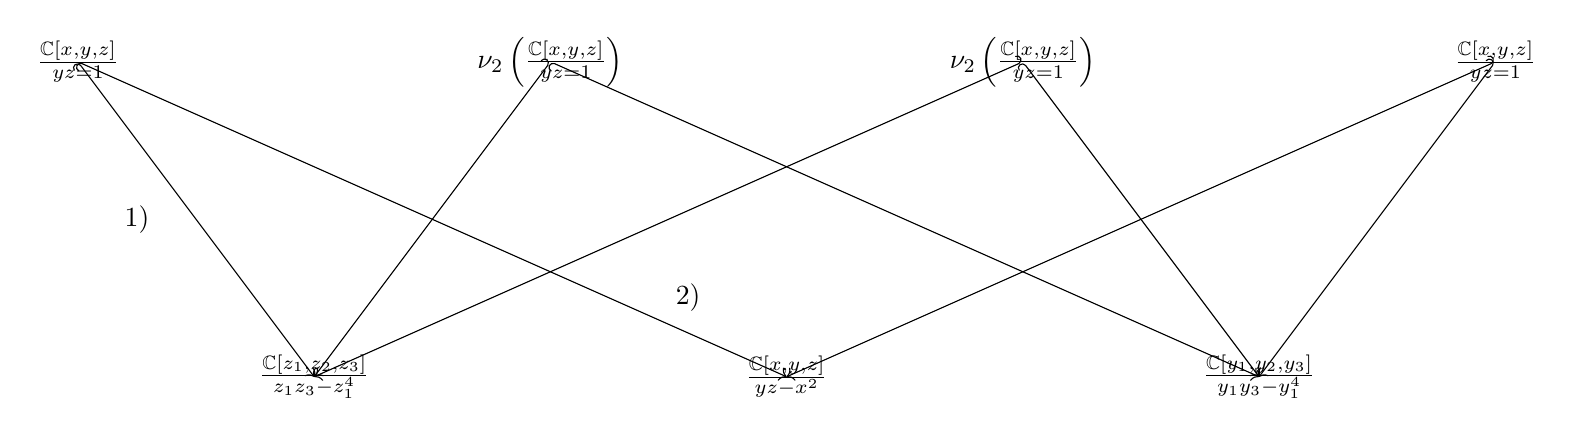
\begin{tikzpicture}
	\begin{pgfonlayer}{nodelayer}
		\node [style=none] (0) at (-6, -4) {};
		\node [style=none] (1) at (0, -4) {$\frac{\mathbb{C}[x,y,z]}{yz-x^2}$};
		\node [style=none] (2) at (6, -4) {$\frac{\mathbb{C}[y_1, y_2, y_3]}{y_1y_3 - y_1^4}$};
		\node [style=none] (3) at (-6, -4) {$\frac{\mathbb{C}[z_1, z_2, z_3]}{z_1z_3 - z_1^4}$};
		\node [style=none] (4) at (-3, 0) {$\nu_2 \left(\frac{\mathbb{C}[x,y,z]}{yz = 1} \right)$};
		\node [style=none] (5) at (3, 0) {$\nu_2 \left(\frac{\mathbb{C}[x,y,z]}{yz = 1} \right)$};
		\node [style=none] (6) at (9, 0) {$\frac{\mathbb{C}[x,y,z]}{yz = 1}$};
		\node [style=none] (7) at (-9, 0) {$\frac{\mathbb{C}[x,y,z]}{yz = 1}$};
		\node [style=none] (8) at (-8.25, -2) {1)};
		\node [style=none] (9) at (-1.25, -3) {2)};
	\end{pgfonlayer}
	\begin{pgfonlayer}{edgelayer}
		\draw [style=new edge style 2] (3.center) to (7.center);
		\draw [style=new edge style 2] (3.center) to (4.center);
		\draw [style=new edge style 2] (3.center) to (5.center);
		\draw [style=new edge style 2] (1.center) to (7.center);
		\draw [style=new edge style 2] (1.center) to (6.center);
		\draw [style=new edge style 2] (2.center) to (4.center);
		\draw [style=new edge style 2] (2.center) to (5.center);
		\draw [style=new edge style 2] (2.center) to (6.center);
	\end{pgfonlayer}
\end{tikzpicture}
\]
We explicitly describe the maps $1)$ and $2)$. To see map $1)$ the base is 
\[
\bigoplus_{m \in M|_{\leq 0}} \mathcal{O}_{\mathbb{P}^1} \left(-mP_0 +\frac{-m}{2} P_1 + \frac{m}{2}P_2 \right) 
\]
and the image is 
\[
\bigoplus_{m \in M} \mathcal{O}_{\mathbb{A}^1}(-mP_0)
\]
There is clearly an inclusion of rings on each level of the negative grading, and this induces the entire map
\end{ex}

We also provide a quick example of when a polyhedral divisor is unmarked but has unmarked subcones cones as the boundary. 

\begin{ex}\rm
Let $N$ be $\mb{Q}^2$. Consider the polyhedral divisor defined by $\delta \otimes P_0 + (1, 1) + \delta \otimes P_1$ over $\mathbb{P}^1$ where $\delta = \langle (1,0) , \, (0, 1) \rangle$. We now insist that two dimensional cone is marked. However if we pick a ray of the tail fan, and calculate the dual we see that this does not satisfy of being semiample on the boundary, if the base curve was non affine.

Upon calculation of the affine ring this can be seen as a toric downgrade of the Atiyah flop, with the quotient corresponding to one of the two natural maps to $\mathbb{P}^1$. To see the two flops the first is by unmarking the two dimensional cone and the other is given by the same polyhedral coefficients but now the tail cone is a tail fan with the ray $(1,1)$ bisecting it. This corresponds to only one of the resolutions resolving the quotient down to the $\mathbb{P}^1$.
\end{ex}


\begin{dfn}
A fansy divisor a smooth curve $C$ is a collection of $n$ subdivison of $\mathbb{Q}$ with markings $\mathbb{Q}^+$, $\mathbb{Q}^-$, $\mathbb{Q}^\pm$ or no markings at all. 
\end{dfn}
This is equivalent to a polyhedral divisor provided the the assumptions of \ref{Tech} are satisfied.
\begin{ex}
One $A_1$ two $A_3$.
\end{ex}

This defines a complexity one surface. In toric varieties full dimensional cones give rise to torus fixed point. Analogously, the same way for varieties of higher complexity every full dimensional subdivision of the plane gives rise to a toric fixed point. In the case of surfaces these fixed points can be classified giving rise to three cases
\begin{itemize}
\item $\bold{Elliptic}$ - Around the fixed point in local coordinates, the torus behaves on all coordinates with positive or negative degree. These points are isolated.
\item $\bold{Parabolic}$ - These always arise as blowups of elliptic points, these occur when in local coordinates, one of the coordinates is acted trivially upon by the torus. These points lie on a section of the map to $Y$
\item $\bold{Hyperbolic}$ - These are where the the local coordinates are acted in positive and negative degree.
\end{itemize}
It is easy to see that Hyperbolic points correspond to a subdivision with $\delta = 0$, Parabolic correspond to an unmarked edge going to infinity and Elliptic to a marked point going to infinity.
\section{Divisors in complexity one}

We now limit ourselves strictly to complexity one, and the chow quotient $Y$ will now be $\mathbb{P}^1$. In the torus setting we know that divisors correspond to rays of the associated fan. Almost exactly the same is true in complexity one: divisors  occur as torus invariant divisor, these correspond the codimension 1 polyhedral divisors or they are premimages of the $\mathbb{P}^1$. These correspond to a polyhedral divisor $\mathcal{D}$  going of to infinity in a direction, with dim$(\delta) = \infty$ which forall $P \in \mathbb{P}^1$ we do not have $\mathcal{D}  |_P = \varnothing$. Note that this also holds for higer dimensions, with a little bit of extra work. From this it is easy to derive the following theorem
\\
\begin{thm}[\cite{PS}]
The Picard rank of a complexity one surface defined by a polyhedral fan $\mathcal{S}$ is 
\[
\rho_X =  \text{ \# Number of parabolic lines } + \sum_{P \in Y} (\# \mathcal{S}_P^{(0)} - 1) 
\]
\end{thm}
where $n$ is the dimension and $\# \mathcal{S}_P^{(0)}$ is the number of points on this slice of the fan. Similar statements can be made in dimension $n$ where the parabolic lines are replaced by x-rays. In a similar style to this we can classify Cartier divisors, we here make no pretense at proof or justification. 
\begin{dfn}
A divisorial support function $h$ on a divisorial fan $\mathcal{S}$ is a piecewise linear function on each component of the fan such that

\begin{itemize}
\item On every polyhedron $\Delta \in \mathcal{S}_{P_i}$ it is a linear function
\item $h$ is continuous
\item at all points $h$ has integer slope and integer translation
\item if $\mathcal{D}_1$ and $\mathcal{D}_2$ have the same tail cone, then the linear part of $h$ restricted to them is equal
\end{itemize}
\end{dfn}
We call a support function principal if it is of the form $h(v) = \langle u, v \rangle + D$, this corresponds to a principal Cartier divisor. We call a support function Cartier, if on every component with complete locus the support function is principal. In the case of Fansy divisors, this just correspond to the edge with a marking. We denote $h$ restricted to a component by $h_P$.  We refer to a piecewise linear function with rational slope and rational translation as a $\mathbb{Q}$ support function.
\begin{thm}[\cite{PS}]
Let $X$ be the variety associated with the divisorial fan $\mathcal{S}$. There exists a one to correspondence between support functions support function quotiented by principal support functions and Cartier divisors on the complexity one variety. In addition there exists 
a one to correspondence between $\mathbb{Q}$ support functions support function quotiented by principal support functions and $\mathbb{Q}$ Cartier divisors on the complexity one variety

\end{thm}
Using the above languages we represent the canonical divisor as a Weil divisor, it has the following form
\begin{thm}[\cite{PS}]
The canonical divisor of a complexity one surface can be represented in the following form
\[
K_X = \sum_{(P, v)} ( \mu (v) K_Y (P) + \mu (v) - 1) \cdot D_{(P,v)} - \sum_\rho D_\rho
\]
\end{thm}
Here $K_Y(P)$ is the degree of $K_Y$ at $P$, and $\mu (v)$ is the smallest value $k$ such that $k \cdot v \in \mathbb{N}$.  While I have not stated the conditions for linear equivalence these can be seen in \cite{PS}, and using these you can show that it does not depend on the choice of representative of $K_Y$. Note that given the singularities and varieties we are working with we know that our $K_X$ will be $\mathbb{Q}$-Cartier. The fano index is clear and easy to derive from the singularities we have, so all that remains is to check on the conditions for a complexity one divisor to be ample.

\begin{thm}[\cite{PS}]
A suppport function $h$ is ample iff for all $P$ we have $h_P$ is strictly concave, and for all polyhedral divisors $\mathcal{D}$ defined on an affine curve we have
\[
- \sum_{P \in \mathbb{P}^1} h_P |_\mathcal{D} (0) \in \text{Weil}_\mathbb{Q} (Y)
\]
 is an ample $\mathbb{Q}$ Cartier divisor.
\end{thm}
Note that in reality $h_P |_\mathcal{D}$ may not be defined at $0$ but we can extend the affine function to $0$. We finish this recap on divisors by describing the Weil divisor corresponding to a Cartier divisor
\begin{thm}[\cite{PS}]
Let $h = \sum_P h_P$ be a Cartier divisor on $\mathcal{S}$ then the corresponding Weil divisor is 
\[
- \sum_\rho h_t ( n_\rho) D_\rho - \sum_{(P, v)} \mu(v) h_P(v) D_{(P,v)}
\]
\end{thm}
Here $n_\rho$ is the generator of the ray inside the tail fan and $\mu(v)$ is as before. Note that is easy to see why we need this $\mu$ function. If you start with a closed subinterval $[a, b]$ and try to work out what the corresponding affine variety is, we see that it just the toric variety defined by the cone $(a,1), \, (b,1)$, and then all you calculations can be done in the realm of toric varieties, however there you use the generator of your rays in the lattice, so you need the $\mu$ function.
\\
\\
We use the above note to easily calulate the minimal resolution of a complexity one surface. Note that we can split this across affine charts, in the first case if we have the affine chart corresponding to the polyhedral divisor $[a,b]$ then using the above point we can can calculate this by the toric methods. In case two where we have a non marked edge going to infinity, we can split this into affine charts $[a_i, \infty)$ this is also a toric chart corresponding to the cone $(a,1), \, (1,0)$, so once again the resolution is toric. The final case is with a marked edge, however we can take a weighted blowup to resolve the ellitic point, then resolve the resulting singularities by the above methods. To calculate the intersection numbers on the resolution you can either use [Tim], \cite{PS} or you can note that the only part that is not toric is the parbolic line, this is defined by glueing together charts coming from $[a_i', \infty)$, here by smootheness $a_i' \in \mathbb{Z}$, this is isomorphic to the charts defined by $[\sum(a_i'), \infty)$ at $P_1$ and $[0, \infty)$ for all other $P_i$. Hence we see that the parabolic line is define torically as the fan  
$(\sum(a_i'), 1), \, (1, 0), \,(0, -1)$ from this an easy derivation of the intersection number follows.
\\
\\
We can also draw out the graph of divisors on the minimal resolution. For example considering the following log del Pezzo from \cite{S}
\[
\left\{-2, 0 \right\} \otimes P_0 + \left\{-\frac{1}{2} \right\} \otimes P_1 + \left\{ -\frac{1}{2} \right\} \otimes P_2 
\]
gives us the following resolution:


\begin{comment}
\begin{figure}[htbp]
\psset{unit=0.95cm}
\begin{pspicture}(0,-8)(12,0)
%\psgrid(0,0)(0,-8)(12,0)
\psframe[linecolor=white](0.5,-10)(3.5,-1.5)

\psline{-}(4,-1.5)(10.5, -1.5)



\psline{-}(6.75,-0.75)(4.5, -3)
\psline[linestyle = dashed]{-}(8.25,-0.75)(6, -3)
\psline{-}(9.75,-0.75)(7.5, -3)
\psline[linestyle = dashed]{-}(5, -2)(5, -5)
\psline{-}(6.5, -2)(6.5, -5)
\psline[linestyle = dashed]{-}(8, -2)(8, -5)
\psline{-}(4.5, -3.75)(6.75,-6.75)
\psline[linestyle = dashed]{-}(6, -3.75)(8.25,-6.75)
\psline{-}(7.5, -3.75)(9.75,-6.75)

\psline{-}(4,-6)(10.5, -6)
\end{pspicture}

\caption{The minimal resolution of the above log del Pezzo. Here the dark lines indicate -2 curves and the dotted lines indicate -1 curves.}

\end{figure}
\end{comment}

\section{Algorithms}
We propose two different algorithms for the classification of complexity one log del Pezzo surfaces. These both rely on several key facts

\begin{lem}{\cite{Suss}}
Let $S$ be a non cyclic complexity one log terminal surface singularity. Then $S$ has, upto isomorphism, a fan over $\mathbb{P}^1$ with coefficients
\[
\left[\frac{p_1}{q_1}, \infty \right) \otimes P_1 + \left[ \frac{p_2}{q_2}, \infty \right) \otimes P_2 + \left[ \frac{p_3}{q_3}, \infty \right) \otimes P_3
\]
with $(q_1, q_2, q_3)$ satisfying $\sum(1 - \frac{1}{q_i}) < 2$.
\end{lem}
\begin{proof}
See \cite{Suss}
\end{proof}
We now use the following crucial lemma
\begin{lem}
Let $S$ be a log terminal surface singularity of Gorenstein index $l$. Let $E$ be an exceptional curve in the minimal resolution. Then $E^2 \geq -2l$ if it is not a trivalent curve and $E^2 \geq -3l$ if it is trivalent.
\end{lem}
\begin{proof}
Via the classification of log terminal singularities \cite{Br} we have that $E$ intersects at most three other exceptional curves. Denote the discrepancies of these curves $d_1, d_2, d_3$, note that any $d_i$ could be equal to zero. Also note that $0 \geq d_i \geq -1$. Denote the discrepancy of $E$ by $d$. Then we have the formula $dE^2 + \sum d_i = 0$.   This rearranges to $d = \frac{(\sum d_i)}{E^2} \leq \frac{-3}{E^2}$ as the singularity is log terminal. As $d \in \frac{1}{l} \mathbb{Z}$ we get $E^2 \geq -3l$. In the case of a non trivalent curve, we can assume $d_3 = 0$ and we see that $E^2 \geq -2l$.
\end{proof}



\begin{lem}
Given a complexity one log del Pezzo surface of index $l$ then there cannot be more than $6l$ points where the polyhedral fan is not the tail fan
\end{lem}
\begin{proof}
Taking the minimal resolution of our log del Pezzo, this admits a map to a Hirzebruch surface $\mathbb{F}_n$. As we are contracting $-1$ curves our map is invariant under the torus action. Hence this is a torus action on the Hirzebruch surface. Any series of complexity one non toric blowups on a toric surface correspond to blowing up points on a line of invariant points. We note that by the above lemma we cannot get a map to $\mathbb{F}_n$ when $n > 3l$. Hence we the largest possible self intersection of a torus invariant curve on our Hirzebruch surface is $3l$ and the smallest possible intersection on our minimal resolution is $-3l$ so there can only be $6l$ blowups on the curve.
\end{proof}

\begin{rem}
In the case of index one, we know DuVal singularities only have $-2$ curves in the resolution hence this bound can be refined to four non general fibers.
\end{rem}

Just as in the case of Gorenstein index one, where the singularities are formed of $-2$ curves. There is an explicit way to classify the resolutions of singularities of higher index.

\begin{lem}[\label{basic bound}]
A singularity of index $n$ which is non toric log terminal singularities can be described by one of the following polyhedral divisors
\begin{itemize}
\item $\left[-\frac{1}{2}, \infty \right) \otimes P_1 + \left[ \frac{1}{2}, \infty \right) \otimes P_2 + \left[ \frac{n}{m}, \infty \right) \otimes P_3$

\item Finite $E_6$, $E_7$, $E_8$ case
\end{itemize}
\end{lem}

\begin{proof}
We note that for the canonical divisor to be Cartier the corresponding slope function has to have integral slope and $h_P(0) \in \mathbb{Z}$ for all $P \in \mb{P}^1$. We note the slope for a polyhedral divisor of the form $\left[-\frac{1}{2}, \infty \right) \otimes P_1 + \left[ \frac{1}{2}, \infty \right) \otimes P_2 + \left[ \frac{p}{q}, \infty \right) \otimes P_3$ is $\frac{1}{p}$. Hence $p$ divides $n$ where $n$ is the index of the singularity. We now note $h_{P_1} (0) = -\frac{-1}{2} + \frac{1}{2} \frac{1}{p} = \frac{1}{2} (1 + \frac{1}{p})$. Now if $p$ is odd this becomes a fraction $\frac{a}{p}$ and if $p$ is even this becomes $\frac{a}{2p}$. Now $h_0(P_3) = \frac{q-1}{q} + \frac{p}{q} \frac{1}{p}$, this is always just $1$. Hence for every $k h_P(n)$ to be an integer for every $P \in \mb{P}^1$ and $n \in \mb{Z}$ we need $k$ to be a multiple of $p$ if $p$ is odd and a multiple of $p$ if $p$ is even.


Do the $E_6, \, E_7,\, E_8$ case.
\end{proof}

\begin{rem}
This imposes stricter bounds on the number of non generic fibers a complexity one surface of index $n$ can have than Lemma~\ref{basic bound} and enables you to put bounds on per the singularity. 
\end{rem}

We also need a bound on what possible toric singularities can occur and the possible actions on them.

\begin{lem}[\label{Structure}]
Let $X$ be a non smooth complexity one log del Pezzo surface with the following properties 
\begin{itemize}
\item $X$ has two elliptic points $P_1$ and $P_2$
\item $X$ has only toric singularities
\item $X$ is non toric
\end{itemize}

Then at least one of the elliptic points, $P_1$, is a singularity.  We can describe $P_1$ locally by a cone $\sigma \subset N \cong \mb{Z}^2$ and a ray $v \in N$. Then $v$ corresponds to a lattice point on the minimal resolution of $\sigma$.
\end{lem}

\begin{proof}
Let $Y$ be the minimal resolution of $X$. Then $X$ admits an equivariant map to $\mb{F}_i$ as every $-1$ curve on $Y$ is torus invariant. Hence $Y$ is constructed by a non toric blowup of a toric surface. Considering the first non toric blowup, we are blowing up a point $P$ on a torus invariant curve $C$. Clearly $C$ is a torus invariant curve in the minimal resolution of $X$. We note that $C$ cannot be a curve on $X$ as otherwise the surface would not have two elliptic points. This proofs the above lemma.


\end{proof}

We finish with the following observation that helps shorten calculations.
Let $X$ be a complexity one surface with the following polyhedral fan:
\[\def\arraystretch{1.2}
\begin{array}{cc}
P_1 & \left[ a_1, \, \dots , \, a_n \right] \\ 
P_2 & \left[b_1 , \, \dots, \, b_m \right] \\
P_3 & \left[c_1, \, \dots, \, c_o, \right] \\
P_4 & \left[d_1, \, \dots, \, d_{p-1}, 0\right]  \\
\end{array}
\]
and a marking $\mb{Q}^+$.
Also assume that the minimal resolution of $X$ contains a curve $E$ which is pointwise fixed by the action and which is contracted to elliptic point at positive infinity.

Let $h$ be the piecewise linear function corresponding to $-K_X$. Then $h_P|_{[0, \, \infty)}$ is defined by a unique value $u \in \mb{Q}$. If $-K_X$ is ample then the only possible values for $d_{p-1}$ are the values $\frac{p}{q}$, with $q >0$, such that $\frac{q-1}{q} < u\frac{p}{q}$. 


As there are a finite number of log del Pezzo surfaces, upto deformation, with Gorenstein index $k$ there can only be a finite number of singularities $S$ which can occur on such a surface. 

\begin{algorithm}

There are two infinte families of singularities of index $k$ corresponding to $A_n$ and $D_n$ singularities. There are then the sporadic cases corresponding to $E_6, \, E_7, \, E_8$.

We start by dealing with the case of two elliptic points as it is the most involved. We start in the case of the $D_n$ singularity. Given $S$ a singularity of index $k$ arising as a $D_n$ quotient, then there is a unique $\mb{C}^\times$ action. The associated polyhedral is given in Lemma~\ref{basic bound} as $\left[-\frac{1}{2}, \infty \right) \otimes P_1 + \left[ \frac{1}{2}, \infty \right) \otimes P_2 + \left[ \frac{k}{n}, \infty \right) \otimes P_3$. Assuming this lies on a log del Pezzo surface we have a polyhedral divisor
\[\def\arraystretch{1.4}
\begin{array}{c}
\left[a_1^1, \, a_2^1,\,  \dots, a_{n_1 - 1}^1, \, \frac{-1}{2} \right] \\
\left[a_1^2, \, a_2^2,\,  \dots, a_{n_2 - 1}^2, \, \frac{1}{2} \right] \\
\left[a_1^3, \, a_2^3,\,  \dots, a_{n_3 - 1}^3, \, \frac{k}{n} \right] \\
\left[a_1^4, \, a_2^4,\,  \dots, a_{n_4}^4 \right] \\
\vdots \\
\left[ a_1^{3k}, \, a_2^{3k}, \,  \dots, a_{n_{3k}}^{3k} \right] \\
\end{array}
\]
We now ask what are the possible values for $\frac{k}{n}$.
\end{algorithm}


As an example we illustrate how this can classify Gorenstein log del Pezzo surfaces which have complexity one.

\begin{ex}\rm

We start with the Gorenstein index $k = 1$, i.e the only singulairties are DuVal. We know there is a singularity which has an action which corresponds to a curve on the minimal resolution. We iterate over all possible singularities and all possible actions until we can show they do not exist. We illustrate this in the case that the singularity with which the action corresponds with a ray in the minimal resolution is an $A_n$ singularity. We assume that this singularity has polyhedral divisor with tail cone $[ 0, \, \infty)$. From now on we assume this without stating it.

To make this easier we make two observations. The first is that if a fiber over a point $P_i$ is $[a_1 = \frac{p_1}{q_1} , \dots, a_n = \frac{p_n}{q_n}, \, 0]$ then $q_i = 1$. This follows via the above remarks, first, we know we get an $A_m$ singularity given by $(0, 1), \, (p_n,  \, q_n)$. Then, via the stated properties of our singularity, we have the slope of $h_P|_{[0, \, \infty)}$ is $-1$. So we need $\frac{q_n-1}{q_n} < \frac{-p_n}{q_n}$ which implies $p_n + q_n < 1$, hence if $q_n > 1$ then $p_n < -1$. Now every point on the line connecting $(p_n, \, q_n)$ to $(0, \, 1)$ has to satisfy this inequality. In particular there is a point $(-1, a)$ on this line, with $a  \in \mb{Z}$, satisfying the inequality, hence $ a \leq 1$. As $ a>0$ for $q_n>0$ we have the only possible value of $a$ is one. This corresponds to $q_n = 1$.


The second observation is let $\mathcal{D} = \frac{1}{u} \otimes P_1 + \frac{1}{v} \otimes P_2$. be a polyhedral divisor with tail cone $[ 0 , \, \infty)$. We can assume without loss of generality that $u \geq v$. Then if $u>v+2$ and $v \geq 2$ then there are no complexity one Gorenstein log del Pezzo surfaces which contain $\mathcal{D}$ as a polyhedral cone. We not as $u,  v \geq 2$ we have the only possible poyhedral fans over $P1$ are $[0, \, \frac{1}{u}
]$ and $[\frac{1}{u}]$, similarly for $P_2$. Viewing this from a toric perspective the only points that can be connected to $(1,u)$ or $(0,1)$ while preserving the necessary convexity are less than $-v$. This implies as a complexity one surface this would need a denominator on another fiber less than $v$, but this cannot happen. 

\begin{itemize}

\item  $A_1$

\item $A_2$

\item $A_3$

\item $A_4$

\item \begin{bf} $A_5$ Singularity \end{bf}

This has several possible actions taking the first us the polyhedral divisor 
\[\def\arraystretch{1.2}
\begin{array}{cc}
P_1 & \left[ a_1, \, \dots , \, a_n, \frac{1}{5} \right] \\ 
P_2 & \left[b_1 , \, \dots, \, b_m, 1\right] \\
P_3 & \left[c_1, \, \dots, \, c_o, 0\right] \\
P_4 & \left[d_1, \, \dots, \, d_p, 0\right]  \\
\end{array}
\]
\end{itemize}
The only choices for the first row are $[0, \frac{1}{5}]$ and $[\frac{1}{5}]$. We call this case $a$ and case $b$. 

In case $a$ if there is another elliptic point it has to be arising from a toric singularity with coordinates $(0, 1)$ and $(-1, u)$ with $u \leq -4$ and the subtorus once again corresponding to the horizontal line.
%Rejig the above sentence.
This cannot happen as every other row can only have denominators equal to $1$. So this case does not occur. Note a non toric singularity cannot occur otherwise the slope on the tailfan $[-\infty , 0)$ would be one and this would not be convex on $P_1$.

For case $b$ we have exactly the same argument that it would have to be connected to a singularity with denominator greater than $1$, hence cannot occur. So this does not occur. 


The next case is 
\[\def\arraystretch{1.2}
\begin{array}{cc}
P_1 & \left[ a_1, \, \dots , \, a_n, \frac{1}{4} \right] \\ 
P_2 & \left[b_1 , \, \dots, \, b_m, \frac{1}{2} \right] \\
P_3 & \left[c_1, \, \dots, \, c_o, 0\right] \\
P_4 & \left[d_1, \, \dots, \, d_p, 0\right]  \\
\end{array}
\]
Once again two cases for $P_1$,  $[0, \frac{1}{4}]$ and $[\frac{1}{4}]$. If it is the first case then the denominator has to be greater than $2$ so does not occur. In the second case there is only one possibility: the other elliptic singularity is given by toric coordinates $(1, \, 4),$ $(-1, -2)$. The only way to get a denominator greater than 1 is on $P_2$ and  the only choice is if this is the original $\frac{1}{2}$ hence we get
\[
\left[\frac{1}{4} \right] \otimes P_1 + \left[\frac{1}{2} \right] \otimes P_2 + [0, -\, 1] \otimes P_3
\]

The final case is 
\[\def\arraystretch{1.2}
\begin{array}{cc}
P_1 & \left[ a_1, \, \dots , \, a_n, \frac{1}{3} \right] \\ 
P_2 & \left[b_1 , \, \dots, \, b_m, \frac{1}{3} \right] \\
P_3 & \left[c_1, \, \dots, \, c_o, 0\right] \\
P_4 & \left[d_1, \, \dots, \, d_p, 0\right]  \\
\end{array}
\]
This leads to a lot more cases, as follows. Once again possible choices for $P_1$ and $P_2$ are $\left[ 0, \, \frac{1}{3} \right]$ or $\left[ \frac{1}{3} \right]$. Once again denoting these by case $a$ and case $b$. In case $a$ it needs to connect to a point with denominator $ u \in \{2, \, 5, \, 8 \dots \}$, however it is impossible to construct any of these denominators, so this does no occur. In the case $b$, we either have the $A_1$ singularity with coordinates $(1, 3),\, (-1, -1)$ or the $A_2$ singularity given by $(1, 3),\, (-2, -3)$, other values result in non compatible denominators. If we had the singularity given by $(1, 3),\, (-1, -1)$, then the polyhedral divisor over $P_2$ would have to be $\left[ 0, \frac{1}{3} \right]$ which we have already shown cannot occur. If we have the $A_2$ singularity then this involves the only way this can be constructed is via 
\[
\left[\frac{1}{3} \right] \otimes P_1 + \left[\frac{1}{3} \right] \otimes P_2 + [0, -\, 1] \otimes P_3
\]
This finishes the $A_5$ case.

\item \begin{bf} $A_N$ Singularity for $N \geq 6$ \end{bf}

This results in a singularity given by surface given by 
\[\def\arraystretch{1.2}
\begin{array}{cc}
P_1 & \left[ a_1, \, \dots , \, a_n, \frac{1}{u} \right] \\ 
P_2 & \left[b_1 , \, \dots, \, b_m, \frac{1}{v} \right] \\
P_3 & \left[c_1, \, \dots, \, c_o, 0\right] \\
P_4 & \left[d_1, \, \dots, \, d_p, 0\right]  \\
\end{array}
\]
We split this into three case 
\begin{enumerate}[label =\alph*)]
\item $u = v$
\item $u = v + 1$
\item $u = v + 2$
\end{enumerate}
Every other case is covered by our discussion at the beginning or the example. We note that which of these cases occur on the value of $N$. We note as $N \geq 6$ this implies $u \geq 4$ and $v \geq 3$.

In case a), the only denominators that occur which are less than or equal to $v$ are $\frac{1}{u-2}$ and $\frac{1}{u-1}$ however as $u \geq 3$, as $N \geq 6$ we have neither of these values are equal to $u$ or $1$ so this cannot occur.

In case b), 
\end{ex}

\begin{ex}
As a Gorenstein surface singularity are of DuVal type we see that the minimal resolution can only admit maps to $\mb{F}_0$, $\mb{F}_1$ or $\mb{F}_2$. We now ask what possible torus actions can there be on these Hirzebruch surfaces such that we will only have DuVal singularities. For convenience we write the fan of $\mb{F}_n$ having rays generated by $(1,0)$, $(0,1)$, $(-1, n)$, $(0,-1)$. We can then write a subtorus as a vector $v \in N$.


We make the observation, to save time, that we have classified all log del Pezzo surfaces which do only admit maps to $\mb{F}_0$ or $\mb{F}_1$ ~\ref{Theroem on curves}. This results in only one surface.


For the case of $\mb{F}_2$ either our torus action coincides with a ray of the fan or it does not. There are only four cases where it coincides. However via symmetry we only need to consider the rays $(0,1)$ and $(1,0)$. In the first case your surface has two parabolic lines and hence admits a well defined map to $\mb{P}^1$. As this a morphism we see that the our torus invariant fibers are $0$ curves. The only ways to blow up a zero curve to get values greater than $-2$ are:
\begin{itemize}
\item $-2$, $-1$, $-2$
\item $-1$, $-2$, \dots , $-2$, $-1$
\item $-1$, $-1$
\item $0$
\end{itemize}
We note that with the exception of the second case nothing there are finitely many options. It is clear that in the second case a chain of $k$ $-2$ curves can only arise on a fiber by blowing up parbolic lines a total of $k+1$ times. However earlier on we showed that there could only be a total of $4$ blowups on the parabolic line hence this is bounded.  


The case of the vector $v = (1,0)$ corresponds to the case of one parabolic line and this case is dealt with in the next paragraphs.


Dealing with the case where the vector $v$ does not correspond to a ray of the fan. To do a non toric blowup we need to do a  sequence of blowups that will produce a line of torus invariant points. We note that if we do this twice then there will be a well defined map to $\mb{P}^1$ with the two parabolic lines being sections. This means that there would be a map to a Hirzerbuch surface such that one of these lines is being sent to the negative section and the other to the positive. As both of these would be fixed by the torus action these have been classified in the previous paragraphs.


In the case we have one parabolic line, this line has to arise as a weighted blowup of a point $P$ which is the intersection of a fiber $F$ and a section $A$. This is because any other torus fixed point would lie on the $-2$ curve, which we would then have to blow up, which would contradict DuVal singularities. Without loss of generality we can assume that our torus fixed point corresponds to cone $(1,0)$, $(0, -1)$. This gives us an affine chart $\mb{A}^2_{x, \, y}$ with the coordinates corresponding to the rays $(1,0)$, $(0, -1)$. The only possible weights are then $(1,1)$, $(2,1)$, $(1,2)$, $(1,3)$ and $(1,-4)$. So the only possible coordinates for $v$ are $(1, -1)$, $(2, -1)$, $(1, -2)$, $(1, -3)$ and $(1,-4)$. We note that if $v = (1,-2)$ is a torus action which also corresponds with a ray, this has a fiber with self intersection $2$. Given a fibration, the fact we can only blow up one side of each fiber means the only possible fibers are of the form 

\begin{itemize}
\item $-1$, $-2$, \dots $-2$ , $n-1$
\item $-2$, $-2$, \dots $-2$, $n-k$
\item $-2$, $-2$, \dots $-2$, $-1$, $-2$

\end{itemize}

The fibres in the other case go have values ranging from $1$ (the $(1,1)$ blowup) to $3$ (the $(2,1)$ weighted blowup). Our analysis can be simplified by noting that after a suitable number of contractions we reach a smooth toric variety which is the minimal resolution of a Gorenstein del Pezzo surface. This results in a massive amount of surfaces, many of which are isomorphic.
However every single one is the minimal resolution of a log del Pezzo surface.

\begin{itemize}
\item Pictures
\end{itemize}

\end{ex}

\begin{rem}
The fact that every surface we produce is the minimal resolution of a log del Pezzo surface in the case that index equals one is unique to this case. This follows from index one singularities having the discrepancy of every curve being equal to zero. In index two it is easy to produce toric surfaces which are not the minimal resolution of a log del Pezzo surface.
\end{rem}


With the above disclaimer we carry on. We know that our standard admit a canonical map to a Hirzebruch surface, so we instead work backwards, take a Hirzebruch surface, look at a subtorus action on it and consider all the ways we can make a basic surface out of it.
\\
From here on out our fan for a Hirzebruch surface $\mathbb{F}_n$ will be $(0,1), \, (1,0), \, (0,-1), \, (-1, n)$. There are 4 possible ways the diagram of the Weil divisors on a Hirzebruch surface with a given $\mathbb{C}^*$ action can look
\begin{enumerate}[label =\Alph*]
\item - Two parabolic lines, this corresponds with the subtorus $(0, \pm 1)$.
\item - One parabolic line, this corresponds to the subtorus $(\pm 1, 0)$.
\item - Two elliptic points, connected by a line, this corresponds the sublattice generated by a point lieing in between $(-1,0)$ and $(-1, n)$.
\item - Two elliptic points, not connected by a line, this corresponds to any other point.
\end{enumerate} 


In the above pictures we have the $n$ curve on the top and the $(-n)$ curve on the bottom, with the two vertical lines being the 0 fibers. The blue lines are parabolic lines, and the red points represent elliptic points.
\\
\\
If $X$ is a log del Pezzo with $Y$ its minimal resolution. The number of Elliptic points can only decrease in the cascade , hence we see that it would map down to one of B, C, D. Next note that if we consider case C or D there is no way to make it non toric without resolving one of the elliptic points. Because of this we have the following theorem 
\\
\begin{thm}
Let $X$ be a complexity one log del Pezzo, $Y$ its minimal resolution. Then if $Y$ has two elliptic points, then $X$ is toric.
\end{thm}
We now split things into a case by case analysis. In case A, we have 0 fibers so we just substitute them with the all possible choices of fibers in\autoref{T:ZDQ}, using \cite{IMT} we know that we can only substitute in at most 4 fibers. Hence this case is finished. Note that actually the 4 fibers comes out in the calculations in this case, although that does not prove the general log del Pezzo case.
\\
\\
 For case B, if we resolve the elliptic point on $Y$ in the process of our cascade then it admits a canoncial $\mathbb{P}^1$ fibration, hence we can factor it through case A. Hence we only care about ones that preserve the elliptic point. From the fan we know that it requires $n$ blowups of $\mathbb{F}_n$ to resolve the elliptic point, in these cases the elliptic point lies on the intersection of a $(-1)$ curve and a curve $C$ with $C^2 > 0$. We also see that the zero curve intersecting the elliptic point has to be taken to one of the cases \autoref{T:ZDQ} , we deal with the three cases, nothing happens at the elliptic point, it becomes an $A_n$ singularity and finally the $[ -2, -1, -2]$. If $n \neq 1,2$ then we cannot have an $A_n$ singularity, as we would have a $(-1)$ curve next to a curve with positive self intersection, i.e  the top line, so we would have to keep on blowing up till it has negative self intersection, but this would resolve the elliptic point. Also note if $n=0$ case B does not occur, it would take zero blowups to resolve the elliptic singularity, i.e we just have two parabolic lines, so it is just case A. We deal with $n=1, \, 2$ separately. In the case of nothing happening at the elliptic point. We need to blow up two point on the parabolic curve to get a non toric surface. After this we have two $(-1)$ intersecting $(-2)$ curves, we know by \autoref{T:ZDQ} there is nothing more we can do at those points, so we are left with only being able to blow up the intersection of a $(-1)$ curve with a positive curve. We know we cannot blow up a third point on the parabolic line or it will stop being a klt singularity.  Moving on to the $[-2, -1, -2]$ case, we have all the same possibilities as before, however it may take slightly less blowups than before we reach an acceptable configuration as we have our elliptic point lieing on a $(-2)$ curve. This leaves with only two non toric options from a given Hirzebruch surface.
\\
\\
In the case of $n=1$ we cannot blowup the elliptic point, the only other difference is not being able to use the klt argument, however the $(-1)$ curve being next to the 0 curve guarantees that it still cannot be less than $(-2)$, and if we modify the $(-1)$ curve in any other way it would arise from a different configuration and hence has already been classified. In the case $n = 2$ it also falls under the previous classifaction as we are only allowed one blowup and in this case the two $(-1)$ curves intersect.
\\
\\
In case C we see there is a symmetry between the two elliptic points, so it does not matter which we resolve. When we resolve it we will have $(-1)$ curve adjacent to at most two sets of negative curves. To make a non toric example, we need to blow up one of the lines connecting the parabolic line to the elliptic point. This curve has self intersection greater than 0, using the same argument as before, we can only blow up one point on the parabolic line. As our curve has positive self intersection we know, that we have to have, by the previous argument again, the following set of curves connecting to our parabolic line $[-2, \, -1, \,  -2, \dots -2 ]$. In particular the number of $-2$ curves is greater than two. Using [Ishii, Brieskhorn] classification of singularities, we see that to be klt, you have to have at most 3 negative meeting in a point and one of those has to be just $-2$ curve. Because of this the possible points generating the torus action, up to symmetry, are 
\\
\begin{itemize}
\item $(n, -1)$ or $(1, -n)$, here this is a $\mathbb{P}(1, n)$ blowup. One component is smooth.
\item $(2n - 1, -2)$ or $(2, -2n+1)$ this weighted blowup gives a $\frac{1}{2}(1,1)$ singularity in one chart, this is the singularity whose resolution is a just a $(-2)$ curve. 
\end{itemize}
Note that different values of $n$ give different singularities in the other chart. In the first case, they are clearly just $A_n$ singularities. In the second case, you just get $[-3, \, -2, \dots -2]$, here the chain has $n-1$ of the $(-2)$ curves. We also need both case of the these torus actions as the vary which side the singularities appear. Of course the Brieskhorn classification is much more comprehensive than this, and once the code is written I will start a more comprehensive check as to which or these give klt log del Pezzos. 
\\
\\
In case D, it proceeds almost exactly the same as case C. However you do not have the pleasantness of the symmetry. However it is still straight forward what will happen, the elliptic point next to $0$ curve and the $n$ curve will have the same possible choices of torus actions as in Case C. For the one on the intersection on the $(-n)$ curve and the 0 curve, 2 of the expected 4 options will not occur due to the presence of the $(-n)$ curve. The Brieskhorn classification in this situation gives us $n \leq 5$.


\begin{comment}
\bibliographystyle{plain}
\begin{thebibliography}{10}

\bibitem{ZDQ}
Z. DeQi:
\newblock{ Logarithmic del Pezzo surfaces of rank one with contractible boundaries}
\newblock{Osaka Journal of Mathematics 25 (1988), 461-497}

\bibitem{Suss} 
H. S{\"u}ss:
\newblock Canonical Divisors on T-Varieties
\newblock{arxiv:0811.0626}

\bibitem{Huggenberger}
E. Huggenberger:
\newblock{ Fano Varieties with Torus Action of Complexity One}
\newblock{Thesis at Universität Tübingen, 2013.}


\bibitem{IMT}
N. Ilten, M. Mishna and C. Trainor:
\newblock{ Classifying Fano Complexity-One T-Varieties via Divisorial Polytopes}
\newblock{To appear in Manuscripta Mathematica}
\newblock{arXiv:1710.04146}

\bibitem{H1}
D. Hwang:
\newblock{ Picard rank one Log del Pezzos}
\newblock{Forthcoming}

\bibitem{H2}
D. Hwang:
\newblock{Cascades of Toric varieties}
\newblock{Unpublished draft version}

\bibitem{Sakai}
F. Sakai:
\newblock{ Anitcanonical models of rational surfaces}
\newblock{Math. Ann. 269 (1984),}
\newblock{no. 3, 389-410.}

\bibitem{CH}
A. Corti and L. Heuberger:
\newblock{ Del Pezzo surfaces with $\frac{1}{3}(1,1)$ points}
\newblock{ Manuscripta Mathematica, May 2017, Volume 152}
\newblock{arXiv:1505.02092}

\bibitem{CP}
D. Cavey and T.Prince:
\newblock{Del Pezzo surfaces with a single 1/k(1,1) singularity,}
\newblock{arXiv:1707.09213}

\bibitem{Altmann}
K. Altmann, N. Ilten, L. Petersen, H. S{\"u}ss and R. Vollmert:
\newblock{ The Geometry of T-Varieties}
\newblock{ 	IMPANGA Lecture Notes, Contributions to Algebraic Geometry, 2012, 17-69}
\newblock{ 	arXiv:1102.5760}

\bibitem{PS}
H. S{\"u}ss:
\newblock{Torus incavriant divisors, }
\newblock{Israel Journal of Mathematics Volume 182 (2011), No. 1, 481-504, }
\newblock{  	arXiv:0811.0517 }

\bibitem{Tim}
A. Timashev:
\newblock{Cartier divisors and geometry of normal G-varieties.}
\newblock{Transform. Groups, 5(2):181–204, 2000.}

\bibitem{Dais}
D. Dais:
\newblock{Toric log del Pezzo surfaces with one singularity}
\newblock{arXiv:1705.06359.}

\bibitem{HP}
D. Hwang and J. Park:
\newblock{Charecterization of log del Pezzo pairs via anticanonical models,}
\newblock{Math. Z. 280 (2015), no 1-2, 211- 229.}

\bibitem{Ishii}
S. Ishii:
\newblock{ Introduction to singularities, }
\newblock{Springer Japan (2014)}

\bibitem{Br}
E. Brieskorn:  
\newblock{Rationale  Singularitäten  komplexer  Flächen.}
\newblock{  Invent.  Math. 4, 336–358 (1968)}

\bibitem{LaurInv}
T. Coates, A. Kasprzyk and T. Prince:
\newblock{Laurent Inversion}
\newblock{ 	arXiv:1707.05842}

\bibitem{Prince}
T. Prince:
\newblock{Smoothing Toric Fano Surfaces Using the Gross-Siebert Algorithm}
\newblock{ Proceedings of the LMS (2018) }

\bibitem{I}
N. Ilten:
\newblock{Mutations of Laurent Polynomials and Flat Families with Toric Fibers}
\newblock{SIGMA, 2012, том 8,	047	(Mi sigma724)}

\bibitem{Port}
I. Portakal:
\newblock{A note on deformations and mutations of fake weighted projective planes}
\newblock{ 	arXiv:1809.04470}

\bibitem{Q}
M. Quereshi:
\newblock{Models of log Del Pezzo surfaces with rigid singularities}
\newblock{ 	arXiv:1711.10222}

\end{thebibliography}
\end{comment}
\end{document} 